%======================================================================
\section{Decision Problem}
\label{sec:decision}
%======================================================================

In this section, we derive structural results characterizing the Stackelberg equilibrium strategy profile $(\varepsilon^*, \mathcal{Z}^*, \mathcal{P}^*)$ under complete information. We establish that finding the firm's optimal response reduces to a finite set of tractable convex optimization subproblems, and show how the regulator optimizes social welfare over the enforcement domain.

\subsection{Firm's Optimal Strategy}

We first characterize the firm's optimal pricing strategy for any given presentation feature $z \in \mathcal{X}$.

\begin{lemma}
\label{lem:pricing}
For a fixed baseline feature $x \in \mathcal{X}$, regulatory enforcement tolerance $\varepsilon \in \mathcal{R}$, and chosen presentation feature $z \in \mathcal{F}_Z(x, \varepsilon)$, the firm's optimal non-negative pricing strategy satisfies $p^*(z) \in \{0\} \cup \{V_j(z) : V_j(z) \ge 0\}$. If all investor valuations are strictly negative ($V_j(z) < 0$ for all $j$), no trade occurs and the firm earns zero capital.
\end{lemma}
\begin{proof}
The proof is given in Section~\ref{sec:proofs_ch5} (Proof~\ref{proof:lem_pricing}).
\end{proof}

Leveraging this structural property of the optimal price, we now characterize the firm's joint presentation and pricing strategy by targeting candidate buyer subpopulations.

\begin{theorem}
\label{thm:firm_opt}
Assume that the subpopulation valuation functions $V_j(z)$ are concave for all $j \in \{1, \dots, k\}$. For any baseline feature $x \in \mathcal{X}$ and enforcement tolerance $\varepsilon \in \mathcal{R}$, the firm's optimal presentation strategy $\mathcal{Z}^*(x, \varepsilon)$ is determined by solving at most $2^k - 1$ constrained convex optimization subproblems (corresponding to non-empty candidate buyer subsets). For fixed small $k$, this yields an exact and tractable reduction to convex programming.
\end{theorem}
\begin{proof} The proof is given in Section~\ref{sec:proofs_ch5} (Proof~\ref{proof:thm_firm_opt}).
\end{proof}

\subsection{Regulator's Optimization and Social Welfare Smoothness}

To determine the optimal enforcement tolerance $\varepsilon^*$, the regulator must anticipate the firm's best-response policy $(\mathcal{Z}^*(X, \varepsilon), \mathcal{P}^*(X, \varepsilon))$ characterized by Theorem~\ref{thm:firm_opt}. We first establish structural properties of the resulting expected social welfare function $\mathcal{W}(\varepsilon)$.

First, we show that social welfare saturates beyond a finite enforcement threshold, effectively compactifying the relevant domain.

\begin{proposition}
\label{prop:saturation}
For the regulatory enforcement domain $\mathcal{R} = [0, \infty)$, expected social welfare $\mathcal{W}(\varepsilon)$ becomes constant for all $\varepsilon$ beyond a finite saturation threshold $\varepsilon_{\max} < \infty$. Consequently, optimizing $\mathcal{W}(\varepsilon)$ over $\mathcal{R}$ is equivalent to optimizing over the compact domain $[0, \varepsilon_{\max}]$.
\end{proposition}
\begin{proof}
The proof is given in Section~\ref{sec:proofs_ch5} (Proof~\ref{proof:prop_saturation}).
\end{proof}

Having established that the effective enforcement domain is compact, we characterize the regulator's optimization problem over expected social welfare $\mathcal{W}(\varepsilon)$.

% \paragraph{Smoothness of Expected Social Welfare.}\phantomsection\label{thm:smoothness}
% Under Assumption~\ref{ass:regularity}, the market distribution admits a smooth probability density function with compact support. When the firm plays its best response $(\mathcal{Z}^*(x, \varepsilon), \mathcal{P}^*(x, \varepsilon))$, the enforcement tolerance $\varepsilon$ enters through the boundary of the feasible presentation set $\mathcal{F}_Z(x, \varepsilon)$, which partitions the feature space into regions where different buyer subsets are targeted. Differentiating the expected social welfare $\mathcal{W}(\varepsilon) = \mathbb{E}_X[W(X, \varepsilon)]$ via Leibniz's rule transfers all derivatives with respect to $\varepsilon$ to boundary evaluations against the smooth feature density. Because the density has compact support and uniformly bounded derivatives of all orders, the expected social welfare function $\mathcal{W}(\varepsilon)$ is infinitely differentiable ($\mathcal{C}^\infty$) on the compact interval $[0, \varepsilon_{\max}]$.

\paragraph{Regulator's Optimization and Tractability}
Anticipating the firm's optimal best-response policy $(\mathcal{Z}^*(X, \varepsilon), \mathcal{P}^*(X, \varepsilon))$ from Theorem~\ref{thm:firm_opt}, the regulator determines the optimal enforcement tolerance by solving:
\begin{equation}
\label{eq:eps_star}
\varepsilon^* \in \arg\max_{\varepsilon \in [0, \varepsilon_{\max}]} \mathcal{W}(\varepsilon).
\end{equation}
Because $\mathcal{W}(\varepsilon)$ is smooth and the domain $[0, \varepsilon_{\max}]$ is compact, finding the global optimum $\varepsilon^*$ reduces to maximizing a continuous, smooth objective over a compact interval. For any specified approximation tolerance $\delta > 0$, compactness guarantees that the domain $[0, \varepsilon_{\max}]$ can be covered by a finite number of $\delta$-balls (or evaluated on a finite grid of mesh size $\delta$), ensuring that $\varepsilon^*$ can be efficiently computed to within tolerance $\delta$ using only finitely many evaluations.


%======================================================================
\subsection{Illustrative Example: Finding optimal regulation for affine valuation functions}
\label{ssec:analytical_proof}
%======================================================================

To characterize optimal regulatory policy, we consider an instance of the IPO problem with $k=2$ investor subpopulations, denoted by $\alpha$ and $\beta$. The market consists of equal population shares ($\pi_\alpha = \pi_\beta = 1/2$), so that $N_\alpha = N_\beta = \mathcal{N}/2$. The feature space $\mathcal{X} \subseteq \mathbb{R}^d$ is convex and compact, with $0$ in its interior. Baseline feature vectors $X \in \mathcal{X}$ are distributed according to a smooth probability density function $f_X(x)$. The personal valuation functions for subpopulations $\alpha$ and $\beta$ are:
\begin{equation}
V_\alpha(z) = w_\alpha^\top z + b_\alpha \quad \text{and} \quad V_\beta(z) = w_\beta^\top z + b_\beta
\end{equation}
respectively. Conditional on baseline realization $X = x$, the true asset value per share $Y \in \mathbb{R}$ realizes as $V_\alpha(x)$ with probability $\gamma(x) \in [0,1]$ and as $V_\beta(x)$ with probability $1 - \gamma(x)$. Furthermore we assume $\eta = 1$, i.e., total number of shares available is $\mathcal{N}$. Let
\begin{equation}
\mu(x) := \mathbb{E}[Y \mid X = x] = \gamma(x) V_\alpha(x) + \bigl(1 - \gamma(x)\bigr) V_\beta(x).
\end{equation} Given regulatory enforcement tolerance $\varepsilon \in [0, \varepsilon_{\max}]$ and baseline feature realization $x \in \mathcal{X}$, the issuing firm selects a presentation vector $z = x + \Delta \in \mathcal{F}_Z(x, \varepsilon) = \{z \in \mathbb{R}^d : \|\Delta\|_2 \le \varepsilon\}$ and posted price $P \ge 0$. From Theorem~\ref{thm:firm_opt}, the firm identifies its optimal response by maximizing capital raised $\Pi_F = P \cdot Q$ across the $2^2 - 1 = 3$ possibilities:
\begin{enumerate}[(i)]
\item Targeting Subpopulation $\alpha$:
  To maximize the perceived valuation of subpopulation $\alpha$, the firm chooses its manipulation vector with $\Delta_\alpha^* = \varepsilon \frac{w_\alpha}{\|w_\alpha\|_2}$. The optimal posted price is
  \begin{equation}
  P_\alpha^*(x, \varepsilon) = V_\alpha(x + \Delta_\alpha^*) = w_\alpha^\top x + b_\alpha + \varepsilon \|w_\alpha\|_2.
  \end{equation}
  At this price, only subpopulation $\alpha$ purchases shares, yielding traded volume $Q_\alpha = N_\alpha = \mathcal{N}/2$. The firm's private capital raised is:
  \begin{equation}
  \Pi_{F,\alpha}(x, \varepsilon) = \frac{\mathcal{N}}{2}\left(w_\alpha^\top x + b_\alpha + \varepsilon \|w_\alpha\|_2\right).
  \end{equation}
  Investors in subpopulation $\alpha$ earn a profit of $\Pi_{I} = Q_\alpha(Y(x) - P_\alpha^*)$. The realized per-capita social welfare is $\frac{\Pi_{F,\alpha} + \Pi_{I}}{\mathcal{N}} = \frac{Q_\alpha Y(x)}{\mathcal{N}} = \frac{1}{2}Y(x)$ and the expected social welfare is $\mathbb{E}[\frac{\mu(x)}{2}]$.
  
\item Targeting Subpopulation $\beta$: Just as in for targetting subpopilation $\alpha$, the firm sets its manipulation vector with $\Delta_\beta^* = \varepsilon \frac{w_\beta}{\|w_\beta\|_2}$, and posts price
  \begin{equation}
  P_\beta^*(x, \varepsilon) = w_\beta^\top x + b_\beta + \varepsilon \|w_\beta\|_2.
  \end{equation}
  Traded volume is $Q_\beta = N_\beta = \mathcal{N}/2$, and the firm raises capital:
  \begin{equation}
  \Pi_{F,\beta}(x, \varepsilon) = \frac{\mathcal{N}}{2}\left(w_\beta^\top x + b_\beta + \varepsilon \|w_\beta\|_2\right).
  \end{equation}
  Investors in subpopulation $\beta$ earn a profit of $\Pi_{I} = Q_\beta(Y(x) - P_\beta^*)$, yielding conditional expected per-capita social welfare $\mathbb{E}[\frac{\mu(x)}{2}]$.
  
\item Targeting Both Subpopulations: Since the entire stock of IPO has to be sold ($Q_{\alpha\beta} = N_\alpha + N_\beta = \mathcal{N}$), both subpopulations must be presented with the same manipulated feature vector $z = x + \Delta \in \mathcal{F}_Z(x, \varepsilon)$. The market-clearing price that induces both groups to purchase is constrained by the lower of their two valuations under the common presentation. Thus, the optimal common price is obtained by solving the max--min program:
  \begin{equation}
  \label{eq:p_alphabeta_simple}
  P_{\alpha\beta}^*(x, \varepsilon) = \max_{\|\Delta\|_2 \le \varepsilon} \min\bigl\{V_\alpha(x + \Delta),\, V_\beta(x + \Delta)\bigr\}.
  \end{equation}
  The firm's capital raised is
  \begin{equation}
  \Pi_{F,\alpha\beta}(x, \varepsilon) = \mathcal{N} P_{\alpha\beta}^*(x, \varepsilon),
  \end{equation}
  and the investors' profit is $\Pi_{I} = \mathcal{N}(Y(x) - P_{\alpha\beta}^*)$. The conditional expected per-capita social welfare is $\frac{\Pi_F + \Pi_{I}}{\mathcal{N}} = \mu(x)$.
\end{enumerate}

\begin{remark}[Optimal Common Presentation for Affine Valuations]
\label{rem:joint_manipulation}
For affine valuations $V_j(z) = w_j^\top z + b_j$, the max--min problem \eqref{eq:p_alphabeta_simple} seeks a common manipulation $\Delta$ satisfying $\|\Delta\|_2 \le \varepsilon$ that maximizes $\min\{w_\alpha^\top(x+\Delta) + b_\alpha,\, w_\beta^\top(x+\Delta) + b_\beta\}$. Posing this as a standard convex program yields the optimal manipulation direction parameterized by a Lagrange multiplier $\lambda \in [0,1]$:
\begin{equation}
\Delta_{\alpha\beta}^* = \varepsilon \frac{\lambda w_\alpha + (1-\lambda) w_\beta}{\|\lambda w_\alpha + (1-\lambda) w_\beta\|_2}.
\end{equation}
When the firm balances both groups ($\lambda = 1/2$), the common manipulation aligns with the angular bisector $\frac{w_\alpha + w_\beta}{\|w_\alpha + w_\beta\|_2}$. Under equal sensitivity norms $\|w_\alpha\|_2 = \|w_\beta\|_2 = w_0$, if $w_\alpha \perp w_\beta$ (orthogonal preferences), the common presentation yields a per-group manipulation gain of $\frac{\varepsilon w_0}{\sqrt{2}}$, reflecting the geometric cost of a shared presentation compared to the separate single-group gain $\varepsilon w_0$.
\end{remark}
The firm's optimal targeting rule partitions the fundamental feature space $\mathbb{R}^d$ into three mutually disjoint decision regions:
\begin{align}
\mathcal{R}_\alpha(\varepsilon) &\triangleq \bigl\{x \in \mathbb{R}^d : \Pi_{F,\alpha}(x,\varepsilon) > \max(\Pi_{F,\beta}(x,\varepsilon),\, \Pi_{F,\alpha\beta}(x,\varepsilon))\bigr\}, \\
\mathcal{R}_\beta(\varepsilon) &\triangleq \bigl\{x \in \mathbb{R}^d : \Pi_{F,\beta}(x,\varepsilon) > \max(\Pi_{F,\alpha}(x,\varepsilon),\, \Pi_{F,\alpha\beta}(x,\varepsilon))\bigr\}, \\
\mathcal{R}_{\alpha\beta}(\varepsilon) &\triangleq \bigl\{x \in \mathbb{R}^d : \Pi_{F,\alpha\beta}(x,\varepsilon) \ge \max(\Pi_{F,\alpha}(x,\varepsilon),\, \Pi_{F,\beta}(x,\varepsilon))\bigr\}.
\end{align}

The expected social welfare is given by:
\begin{equation}
\label{eq:welfare_simplified}
\begin{aligned}
\mathcal{W}(\varepsilon) &= \int_{\mathcal{R}_\alpha(\varepsilon)} \frac{1}{2} \mu(x) f_X(x) \, dx + \int_{\mathcal{R}_\beta(\varepsilon)} \frac{1}{2} \mu(x) f_X(x) \, dx + \int_{\mathcal{R}_{\alpha\beta}(\varepsilon)} 1 \cdot \mu(x) f_X(x) \, dx\\
&= \frac{1}{2} \mathbb{E}[\mu(X)] + \frac{1}{2} \int_{\mathcal{R}_{\alpha\beta}(\varepsilon)} \mu(x) f_X(x) \, dx.
\end{aligned}
\end{equation}
The regulation level $\varepsilon$ influences social welfare exclusively through the set $\mathcal{R}_{\alpha\beta}(\varepsilon) = \bigl\{x \in \mathbb{R}^d : \Pi_{F,\alpha\beta}(x,\varepsilon) \ge \max(\Pi_{F,\alpha}(x,\varepsilon),\, \Pi_{F,\beta}(x,\varepsilon))\bigr\}$. We now characterise this set into two sectors.
\begin{enumerate}[(a)]
\item When $P_\alpha^*(x, \varepsilon) \ge P_\beta^*(x, \varepsilon)$, we have $P_{\alpha\beta}^* = P_\beta^*$. The firm prefers serving both groups over targeting group $\alpha$ alone if and only if $\Pi_{F,\alpha\beta} \ge \Pi_{F,\alpha} \iff \mathcal{N} P_\beta^* \ge \frac{\mathcal{N}}{2} P_\alpha^*$, which yields the linear half-space condition
  \begin{equation}
  \label{eq:halfspace_alpha}
  \left(w_\beta^\top x + b_\beta + \varepsilon \|w_\beta\|_2\right) - \frac{1}{2}\left(w_\alpha^\top x + b_\alpha + \varepsilon \|w_\alpha\|_2\right) = a_\alpha^\top x - c_\alpha + \rho_\alpha \varepsilon \ge 0,
  \end{equation}
  where
  \begin{equation}
  \label{eq:params_alpha}
  a_\alpha := w_\beta - \frac{1}{2}w_\alpha \in \mathbb{R}^d, \qquad c_\alpha := \frac{1}{2}b_\alpha - b_\beta \in \mathbb{R}, \qquad \rho_\alpha := \|w_\beta\|_2 - \frac{1}{2}\|w_\alpha\|_2 \in \mathbb{R}.
  \end{equation}

\item When $P_\beta^*(x, \varepsilon) > P_\alpha^*(x, \varepsilon)$, we have $P_{\alpha\beta}^* = P_\alpha^*$. The condition $\Pi_{F,\alpha\beta} \ge \Pi_{F,\beta} \iff \mathcal{N} P_\alpha^* \ge \frac{\mathcal{N}}{2} P_\beta^*$ similarly gives
  \begin{equation}
  \label{eq:halfspace_beta}
  \left(w_\alpha^\top x + b_\alpha + \varepsilon \|w_\alpha\|_2\right) - \frac{1}{2}\left(w_\beta^\top x + b_\beta + \varepsilon \|w_\beta\|_2\right) = a_\beta^\top x - c_\beta + \rho_\beta \varepsilon \ge 0,
  \end{equation}
  where
  \begin{equation}
  \label{eq:params_beta}
  a_\beta := w_\alpha - \frac{1}{2}w_\beta \in \mathbb{R}^d, \qquad c_\beta := \frac{1}{2}b_\beta - b_\alpha \in \mathbb{R}, \qquad \rho_\beta := \|w_\alpha\|_2 - \frac{1}{2}\|w_\beta\|_2 \in \mathbb{R}.
  \end{equation}
\end{enumerate}
Thus $\mathcal{R}_{\alpha\beta}(\varepsilon)$ partitions into two disjoint boundary sectors $\mathcal{R}_{\alpha\beta}(\varepsilon) = \mathcal{R}_{\alpha\beta,\alpha}(\varepsilon) \cup \mathcal{R}_{\alpha\beta,\beta}(\varepsilon)$, where
\begin{align}
\mathcal{R}_{\alpha\beta,\alpha}(\varepsilon) &:= \left\{x \in \mathbb{R}^d : a_\alpha^\top x \ge c_\alpha - \rho_\alpha \varepsilon\right\} \cap C_\alpha, \\
\mathcal{R}_{\alpha\beta,\beta}(\varepsilon) &:= \left\{x \in \mathbb{R}^d : a_\beta^\top x \ge c_\beta - \rho_\beta \varepsilon\right\} \cap C_\beta,
\end{align}
with price-ordering sectors $C_\alpha := \{x \in \mathbb{R}^d : P_\alpha^*(x, \varepsilon) \ge P_\beta^*(x, \varepsilon)\}$ and $C_\beta := \{x \in \mathbb{R}^d : P_\beta^*(x, \varepsilon) > P_\alpha^*(x, \varepsilon)\}$. Under equal biases $b_\alpha = b_\beta = b_0$ and equal sensitivity norms $\|w_\alpha\|_2 = \|w_\beta\|_2 = w_0$, these sectors simplify to $C_\alpha = \{x : (w_\alpha - w_\beta)^\top x \ge 0\}$ and $C_\beta = \{x : (w_\alpha - w_\beta)^\top x < 0\}$, which are static and form a partition of the feature space $\mathcal{X}$.

Let $S_j := a_j^\top X \in \mathbb{R}$ denote the scalar random variable with marginal probability density function $f_{S_j}(s)$. Defining the sector-restricted conditional expected valuation as $\bar{\mu}_j(s) := \mathbb{E}[\mu(X)\mathbf{1}_{C_j}(X) \mid S_j = s]$, the Law of Iterated Expectations yields
\begin{equation}
\label{eq:lie_disintegration_step}
\int_{\mathcal{R}_{\alpha\beta, j}(\varepsilon)} \mu(x) f_X(x) \, dx = \mathbb{E}\Bigl[\mu(X) \mathbf{1}_{C_j}(X) \mathbf{1}_{\{S_j \ge c_j - \rho_j \varepsilon\}}\Bigr] = \int_{c_j - \rho_j \varepsilon}^\infty \bar{\mu}_j(s) f_{S_j}(s) \, ds.
\end{equation}
Because $C_\alpha \cap C_\beta = \emptyset$ and $C_\alpha \cup C_\beta = \mathcal{X}$, upon full saturation when $c_j - \rho_j \varepsilon \le s_{\min, j}$ for both sectors, $\sum_{j \in \{\alpha, \beta\}} \int_{-\infty}^\infty \bar{\mu}_j(s) f_{S_j}(s) \, ds = \mathbb{E}[\mu(X)(\mathbf{1}_{C_\alpha}(X) + \mathbf{1}_{C_\beta}(X))] = \mathbb{E}[\mu(X)]$, cleanly verifying the full-sale limit without double counting. Substituting into~\eqref{eq:welfare_simplified}, we obtain expected social welfare as
\begin{equation}
\label{eq:welfare_1d_disintegration}
\mathcal{W}(\varepsilon) = \frac{1}{2} \mathbb{E}[\mu(X)] + \frac{1}{2} \sum_{j \in \{\alpha, \beta\}} \int_{c_j - \rho_j \varepsilon}^{\infty} \bar{\mu}_j(s) f_{S_j}(s) \, ds.
\end{equation}
Since $\varepsilon$ appears solely in the lower limit of integration, the Fundamental Theorem of Calculus yields
\begin{align}
\label{eq:w_prime_full}
\mathcal{W}'(\varepsilon) &= \frac{1}{2} \sum_{j \in \{\alpha, \beta\}} \rho_j \cdot \bar{\mu}_j(c_j - \rho_j \varepsilon) \cdot f_{S_j}(c_j - \rho_j \varepsilon), \\
\label{eq:w_double_prime_full}
\mathcal{W}''(\varepsilon) &= -\frac{1}{2} \sum_{j \in \{\alpha, \beta\}} \rho_j^2 \left[ \bar{\mu}_j'(c_j - \rho_j \varepsilon) f_{S_j}(c_j - \rho_j \varepsilon) + \bar{\mu}_j(c_j - \rho_j \varepsilon) f_{S_j}'(c_j - \rho_j \varepsilon) \right].
\end{align}


\paragraph{Simplification under Equal Biases and Equal Weight Norms}
To characterize the qualitative behavior of optimal regulation, we assume equal baseline biases $b_\alpha = b_\beta = b_0 \in \mathbb{R}$ and equal sensitivity norms $\|w_\alpha\|_2 = \|w_\beta\|_2 = w_0 > 0$ with $w_\alpha \neq w_\beta$. This assumption implies $c_\alpha = c_\beta = c := -\frac{1}{2} b_0$ and $\rho_\alpha = \rho_\beta = \rho := \frac{1}{2} w_0 > 0$. Recall that the feature space $\mathcal{X}$ is convex and compact with $0 \in \mathrm{int}(\mathcal{X})$ and $a_j \neq 0$, therefore each random variable $S_j = a_j^\top X$ has bounded support $[s_{\min, j}, s_{\max, j}]$, where $s_{\min, j} := \min_{x \in \mathcal{X}} a_j^\top x < 0$ and $s_{\max, j} := \max_{x \in \mathcal{X}} a_j^\top x > 0$. For each boundary sector, the lower integration limit $c - \rho \varepsilon$ sweeps across the support of $S_j$ as $\varepsilon$ increases. By Proposition~\ref{prop:saturation}, expected social welfare saturates once $c - \rho \varepsilon \le s_{\min, j}$ for all $j \in \{\alpha, \beta\}$, thus $\varepsilon_{\max} = \max_{j\in\{\alpha,\beta\}} ((c - s_{\min, j})/\rho) < \infty$. Therefore, the expected welfare and its derivatives simplify to
\begin{align}
\mathcal{W}(\varepsilon) &= \frac{1}{2}\mathbb{E}[\mu(X)] + \frac{1}{2}\sum_{j\in\{\alpha,\beta\}} \int_{c - \rho \varepsilon}^{s_{\max, j}} \bar{\mu}_j(s) f_{S_j}(s)\,ds, \\
\mathcal{W}'(\varepsilon) &= \frac{\rho}{2} \sum_{j\in\{\alpha,\beta\}} \bar{\mu}_j(c - \rho \varepsilon) f_{S_j}(c - \rho \varepsilon), \label{eq:w_prime_reduced} \\
\mathcal{W}''(\varepsilon) &= -\frac{\rho^2}{2} \sum_{j\in\{\alpha,\beta\}} \left[ \bar{\mu}_j'(c - \rho \varepsilon) f_{S_j}(c - \rho \varepsilon) + \bar{\mu}_j(c - \rho \varepsilon) f_{S_j}'(c - \rho \varepsilon) \right].
\end{align}

We now establish a sufficient condition for $\mathcal{W}(\varepsilon)$ to be optimal at an interior point.

\begin{proposition}[Non-monotonicity of the welfare function]
\label{prop:interior_optimality}
Let baseline feature space $\mathcal{X} \subset \mathbb{R}^d$ be compact and convex with $0 \in \mathrm{int}(\mathcal{X})$. Assume equal biases $b_\alpha = b_\beta = b_0$, equal sensitivity norms $\|w_\alpha\|_2 = \|w_\beta\|_2 = w_0 > 0$, and marginal densities satisfy $f_{S_j}(s) > 0$ on $(s_{\min, j}, s_{\max, j})$. If the conditional expected valuation functions $\bar{\mu}_j(s) := \mathbb{E}[\mu(X) \mid S_j = s]$ satisfy
\begin{enumerate}[(i)]
    \item Strict monotonicity: $\bar{\mu}_j'(s) > 0$ for all $s \in [s_{\min, j}, s_{\max, j}]$ and each $j \in \{\alpha, \beta\}$,
    \item Viability at baseline cutoff: $\bar{\mu}_j(c) > 0$ for each $j \in \{\alpha, \beta\}$, where $c = -\frac{1}{2}b_0$,
    \item Non-viability of lowest baseline features: $\bar{\mu}_j(s_{\min, j}) < 0$ for each $j \in \{\alpha, \beta\}$,
\end{enumerate}
then the optimal regulatory enforcement policy $\varepsilon^*$ lies strictly in the interior of the enforcement domain, $\varepsilon^* \in (0, \varepsilon_{\max})$, satisfying $\mathcal{W}'(\varepsilon^*) = 0$.
\end{proposition}
\begin{proof} The proof is given in Section~\ref{sec:proofs_ch5} (Proof~\ref{proof:prop_interior_optimality}).
\end{proof}

\paragraph{Verification of Non-Emptiness}
To confirm that the sufficient conditions of Proposition~\ref{prop:interior_optimality} are non-empty, consider a 2D market instance with equal baseline biases $b_\alpha = b_\beta = 1$ (so $c = -\frac{1}{2}$) and orthogonal investor sensitivity vectors $w_\alpha = (2, 0)^\top$ and $w_\beta = (0, 2)^\top$, so that $\|w_\alpha\|_2 = \|w_\beta\|_2 = 2$ and $\rho = 1$. The investor valuations are $V_\alpha(x) = 2x_1 + 1$ and $V_\beta(x) = 2x_2 + 1$. Assuming equal mixture probabilities $\gamma_\alpha = \gamma_\beta = 1/2$, the true fundamental expected valuation is the valid convex combination $\mu(x) = \frac{1}{2}V_\alpha(x) + \frac{1}{2}V_\beta(x) = x_1 + x_2 + 1$. The vectors $a_\alpha = (-1, 2)^\top$ and $a_\beta = (2, -1)^\top$ define the scores $S_\alpha = -X_1 + 2X_2$ and $S_\beta = 2X_1 - X_2$, which satisfy $S_\alpha + S_\beta = X_1 + X_2$. We define the feature space as the compact convex domain $\mathcal{X} = \{x \in \mathbb{R}^2 : -3 \le -x_1 + 2x_2 \le 3 \text{ and } -3 \le 2x_1 - x_2 \le 3\}$ with uniform distribution $X \sim U(\mathcal{X})$. Because this linear transformation maps $\mathcal{X}$ bijectively onto the product domain $[-3, 3]^2$, the variables $S_\alpha$ and $S_\beta$ are independent uniform random variables on $[-3, 3]$ with support bounds $s_{\min} = -3 < 0 < 3 = s_{\max}$ and saturation threshold $\varepsilon_{\max} = c - s_{\min} = 2.5$. Within each symmetric sector, $\bar{\mu}_j(s) = \frac{1}{2}(s + \mathbb{E}[S_{j'}]) + \frac{1}{2} = \frac{1}{2}s + \frac{1}{2}$. This directly satisfies all three conditions: (i) $\bar{\mu}_j'(s) = 1/2 > 0$, (ii) $\bar{\mu}_j(c) = \bar{\mu}_j(-0.5) = 0.25 > 0$, and (iii) $\bar{\mu}_j(-3) = -1 < 0$. Solving $\mathcal{W}'(\varepsilon^*) = 0$ yields the unique interior optimal enforcement policy $\varepsilon^* = 2.0 \in (0, 2.5)$, with $\mathcal{W}''(\varepsilon^*) < 0$, confirming strict concavity and global interior maximality.


% Applied Fix: Corrected joint presentation price to max-min formulation and recalculated conditional means.

We extend beyond the linear setting by conducting Monte Carlo simulations ($5{,}000$ independent market realizations per enforcement level $\varepsilon$, $\pm 1$ standard error bands)\coderef{subsec:code_ipo_decision} with logistic valuation functions:
\begin{equation}
  V_j(z) = \sigma(u_j + v_j z), \quad \sigma(s) = \frac{1}{1+e^{-s}}.
\end{equation}
We fix $N_1=N_2=50$, $\eta=1$, $X\sim U[-1,1]$, and Group~1 parameters at $u_1=0$, $v_1=+4$ throughout. Group~2 parameters are varied across two parameter families:

\begin{enumerate}
  \item[(i)] \textit{$\gamma$-Sweep (Panels~(a) and~(b), Figure~\ref{fig:decision_sim}):} $u_2=0$ fixed; $v_2 \in \{-8,-6,-4,-2,+2\}$.
  \item[(ii)] \textit{$\delta$-Sweep (Panels~(c) and~(d), Figure~\ref{fig:decision_sim}):} $v_2=-4$ fixed; $u_2 \in \{-4,-2,0,+2,+4\}$.
\end{enumerate}

Figure~\ref{fig:decision_sim} displays the simulation results, illustrating the non-monotonic trajectory of expected social welfare alongside expected firm capital in representative instances, as well as the asymptotic saturation of curves as $\varepsilon$ increases across all configurations, empirically corroborating our theoretical findings.

\begin{figure}[t]
\centering
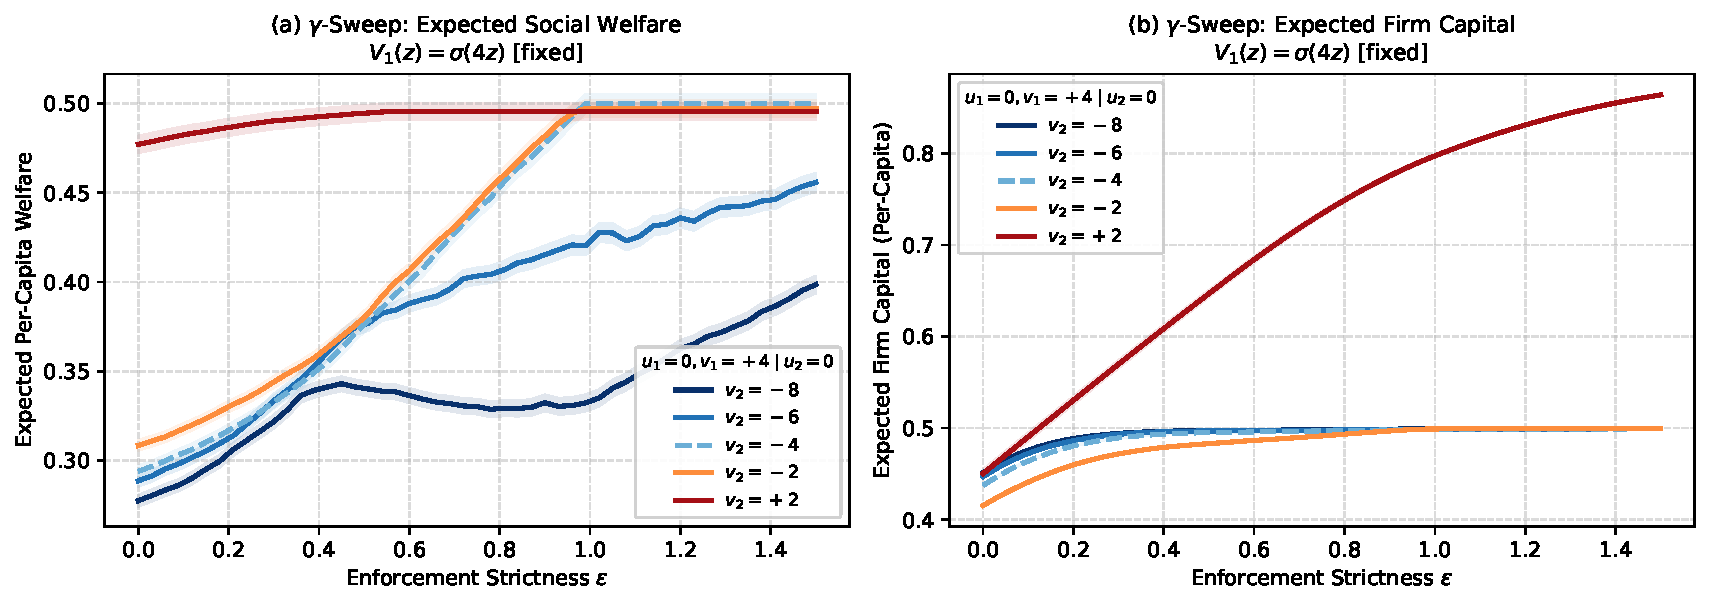
\includegraphics[width=\textwidth]{figures/decision_sim_results.pdf}
\caption{Decision problem simulation across the $\gamma$-sweep and $\delta$-sweep.}
\label{fig:decision_sim}
\end{figure}
